% !TEX root = EUDAQUserManual.tex
\section{Run an Example Setup}
This section will describe running the DAQ system, mainly from the point of view of running an example setup as a demonstration without dedicated hardware.
However, this description can be applied to a detector DAQ system in general.

\subsection{Target Setup}
In this example, a user hardware device is simulated and implemented as an example Producer which can be configured to generate fake data. This works similarly to a real Producer, but does not talk to any real hardware. An example DataCollector is also implemented. \\
The runtime setup consists of the following EUDAQ processes.
\begin{description}
\ttitem{RunControl}
an example RunControl instanced by GUI application.
\ttitem{LogCollector}
a default LogCollector instanced by GUI application.
\ttitem{Producer}
Two example Producers instanced by the CLI command. Both of them produces events at a rate of 1\,Hz, they may have time offset of start run.
\ttitem{DataCollector}
an example DataCollectors instanced by the CLI command.
\ttitem{Monitor}
an example monitor which prints out the asambled Event from the DataCollector in the command line terminal.
\end{description}

\subsection{Preparation}
Some preparation is needed to make sure the environment is set up correctly and
the necessary TCP ports are not blocked before the DAQ can run properly.

\subsubsection{Directories}
If no specified path is passed to EUDAQ (by configuration file or command line parameter), EUDAQ will assume the working folder where executable is started up is writable. Data and log files will be stored in the working folder.

\subsubsection{Init/Config-Files}\label{sec:ConfigFiles}
\texttt{$\ast$.ini}-files for initialization and \texttt{$\ast$.conf}-files for configuration
are text files in a specific format, containing name-value pairs separated into different sections.\footnote{\url{https://en.wikipedia.org/wiki/INI\_file}}
Any text from a \texttt{\#} character until the end of the line is treated as a comment, and
ignored.  
Each section in the config file is delimited by a pair of names seperated by a perioid in square brackets (e.g. \verb@[Producer.Example]@).
The name before peroid represents the type of process to which it applies, the one after peroid is the runtime name of the applied process.
. There is an exception, the section for Run Control is always \verb@[RunControl]@ in which there is no runtime name. 
Within each section, any number of parameters may be specified,
in the form \mbox{\texttt{Name = Value}}.  The EUDAQ native supported parmaters have a common prefix \texttt{EUDAQ\_}.
It is then up to the individual processes how these parameters are interpreted.

During the initialization and configuration, each process gets its section and does not know about the other parts of the ini/conf files.
\myinputlisting[conf]{-30}{user/example/misc/Ex0.ini}

\myinputlisting[conf]{-30}{user/example/misc/Ex0.conf}

\subsubsection{Ports and Firewall}
The different processes communicate between themselves using TCP/IP sockets. The ports can be configured when calling the the processors on the command line (see below). By default, TCP port 44000 is listened to by the RunControl, and TCP port 44002 is listened to by the LogCollector to get connections from clients. The DataCollector will pick a random TCP port to listen to and get incoming data from its connected Producers if there is no specific port assigned explicitly by user.

When all EUDAQ processes run on the same computer, common firewalls will not affect the TCP connections among them. However, running EUDAQ distributively on several computers may have issue from firewall blocking. You will have to open up those TCP ports for incoming connections, temporally shut down the firewall. Shutting down the firewall is operating-system dependent.\\

In this example, all processes will run on the same Linux computer, so we can skip the setup of TCP port.

%%%%%%%%%%%%%%%%%%%%%%%%%%%%%%%%%%%%%%%%%%%%%%%%%%%%%%%%%%%%%%%55
\subsection{Startup}
To start EUDAQ, all of the necessary processes have to be started in the correct order.
The first process must be the Run Control,
since all other processes will attempt to connect to it when they start up.
Then it is recommended to start the Log Collector,
since any log messages it receives may be useful
to help with debugging in case everything does not start as expected.
Finally, the Data Collector, Producers and Monitor can be started in any order you want.

\subsubsection{RunControl}
\label{sec:runcontrol}
There are two versions of the RunControl -- a text-based version \texttt{euCliRun} and a graphical version \texttt{euRun} (see \autoref{fig:RunControl}).

The command line pattern to start up a Log Collector is:
\begin{listing}[mybash]
$[euRun]$ -n {code_name} -a tcp://{listening_port}
\end{listing}

\begin{description}
\ttitem{-n \param{code\_name}}
optional, if it is not specified, default RunControl will be instanced. 
\ttitem{-a \param{listening\_addr}}
optional, \texttt{listening\_port} default value is 44000.
\end{description}

For this example setup, we will startup the euRun GUI which internally instances the default Run Control and make it serve at TCP port 44000:\\
\begin{listing}[mybash]
$[euRun]$ -n Ex0RunControl -a tcp://44000
\end{listing}

After executing the above command, a new GUI windows is shown in \autoref{fig:RunControl}.
\begin{figure}[htb]
  \begin{center}
    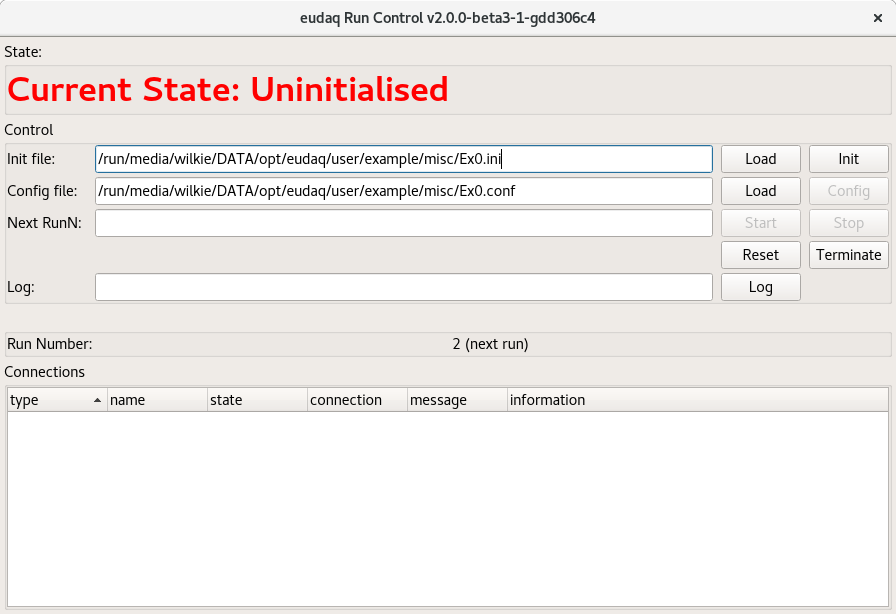
\includegraphics[width=0.8\textwidth]{src/images/eurun_ui}
    \caption{The Run Control graphical user interface.}
    \label{fig:RunControl}
  \end{center}
\end{figure}

\paragraph{Initialization Section}
\begin{listing}[conf]
[RunControl]
# The Ex0RunControl does not need any paramters.
\end{listing}

\paragraph{Configuration Section}
\begin{listing}[conf]
[RunControl]
EX0_STOP_RUN_AFTER_N_SECONDS = 60
\end{listing}

\subsubsection{LogCollector}
\label{sec:logcollector}
It is recommended to start the Log Collector directly after having started the Run Control and before starting other processors in order to collect all log messages generated by all other processes.

There are also two versions of the Log Collector.
The graphical version is called \texttt{euLog},
and the text-based version is called \texttt{euCliLogger}.

The command line pattern to startup a Log Collector is:
\begin{listing}[mybash]
$[euLog]$ -r tcp://{run_contorl_hostname}:{run_contorl_port} -a tcp://{listening_port}
\end{listing}

\begin{description}
\ttitem{-r \param{runcontrol\_addr}}
optional, \texttt{run\_control\_hostname} default value: localhost;  \texttt{run\_contorl\_port}  default value: 44000.
\ttitem{-a \param{listening\_addr}}
optional, \texttt{listening\_port} default value is 44002.
\end{description}

For this example setup, we will startup the GUI version of Log Collector, connect it to the Run Contorl at local port 44000 and make it serve at TCP port 44002:\\
\begin{listing}[mybash]
$[euLog]$ -r tcp://localhost:44000 -a tcp://44002
\end{listing}

After executing the above command, a new GUI window, as shown in \autoref{fig:LogCollector}, is opened and the RunControl displays a new connection, as seen in \autoref{fig:RunControl_con_log}.
\begin{figure}[htb]
  \begin{center}
    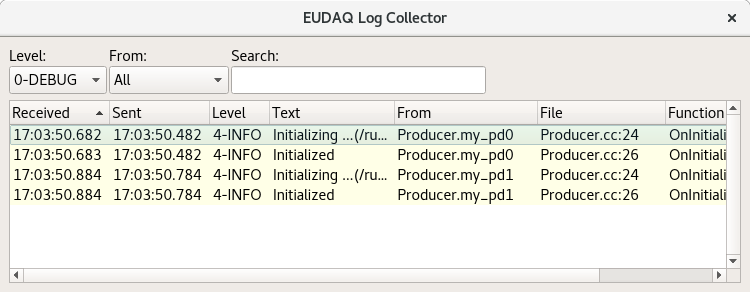
\includegraphics[width=\textwidth]{src/images/eulog_ui}
    \caption{The Log Collector graphical user interface.}
    \label{fig:LogCollector}
  \end{center}
\end{figure}


\paragraph{Initialization Section}
\begin{listing}[conf]
[LogCollector.log]
# Currently, all LogCollectors have a hardcoded runtime name: log
EULOG_GUI_LOG_FILE_PATTERN = myexample_$12D.log
# the $12D will be converted a data/time string with 12 digits. 
\end{listing}

\paragraph{Configuration Section}
\begin{listing}[conf]
[LogCollector.log]
# Currently, all LogCollectors have a hardcoded runtime name: log
# nothing
\end{listing}

\subsubsection{DataCollector}
\label{sec:datacollector}
There is only a text-based version called \texttt{euCliCollector}.
The command line pattern to startup a DataCollector is:
\begin{listing}[mybash]
$[euCliCollector]$ -n {code_name} -t {runtime_name} -r tcp://{run_control_hostname}:{run_contorl_port} -a tcp://{listening_port}
\end{listing}

\begin{description}
\ttitem{-n \param{code\_name}}
required.
\ttitem{-t \param{runtime\_name}}
required.
\ttitem{-r \param{runcontrol\_addr}}
optional, \texttt{run\_control\_hostname} default value: localhost;  \texttt{run\_contorl\_port}  default value: 44000.
\ttitem{-a \param{listening\_addr}}
optional, \texttt{listening\_port} default value is random.
\end{description}

By default, an example DataCollector \texttt{Ex0TgDataCollector} is available with the standard installation of EUDAQ.
For this example setup, we will startup two instances of \texttt{Ex0TsDataCollector} with runtime names \texttt{my\_dc} and \texttt{another\_dc}\\
\begin{listing}[mybash]
$[euCliCollector]$ -n Ex0TgDataCollector -t my_dc -r tcp://localhost:44000 -a tcp://45001
\end{listing}

\paragraph{Initialization Section}
\begin{listing}[conf]
[DataCollector.my_dc]
# nothing
\end{listing}

\paragraph{Configuration Section}
\begin{listing}[conf]
[DataCollector.my_dc]
EUDAQ_MN=my_mon
# send assambled event to the monitor with runtime name my_mon;
EUDAQ_FW=native
# the format of data file
EUDAQ_FW_PATTERN=$12D_run$6R$X
# the name pattern of data file
# the $12D will be converted a data/time string with 12 digits.
# the $6R will be converted a run number string with 6 digits.
# the $X will be converted the suffix name of data file.
\end{listing}

\subsubsection{Producer}
\label{sec:testproducer}
There is only a text-based version called \texttt{euCliProducer}.
The command line pattern to startup a Producer is:
\begin{listing}[mybash]
$[euCliProducer]$ -n {code_name} -t {runtime_name} -r tcp://{run_control_hostname}:{run_contorl_port}
\end{listing}

\begin{description}
\ttitem{-n \param{code\_name}}
required.
\ttitem{-t \param{runtime\_name}}
required.
\ttitem{-r \param{runcontrol\_addr}}
optional, \texttt{run\_control\_hostname} default value: localhost;  \texttt{run\_contorl\_port}  default value: 44000.
\end{description}

By default, an example Producer \texttt{Ex0Producer} is available with the standard installation of EUDAQ.
For this example setup, we will startup two instances of \texttt{Ex0Producer} with runtime names \texttt{my\_pd0} and \texttt{my\_pd0}\\
\begin{listing}[mybash]
$[euCliProducer]$ -n Ex0Producer -t my_pd0 -r tcp://localhost:44000
$[euCliProducer]$ -n Ex0Producer -t my_pd1 -r tcp://localhost:44000
\end{listing}

\paragraph{Initialization Section}
\begin{listing}[conf]
[Producer.my_pd0]
EX0_DEV_LOCK_PATH = /tmp/mydev0.lock

[Producer.my_pd1]
EX0_DEV_LOCK_PATH = /tmp/mydev1.lock
\end{listing}

\paragraph{Configuration Section}
\begin{listing}[conf]
[Producer.my_pd0]
EUDAQ_DC=my_dc
EX0_PLANE_ID=0
EX0_DURATION_BUSY_MS=1
EX0_ENABLE_TRIGERNUMBER=1

[Producer.my_pd1]
EUDAQ_DC=my_dc
EX0_PLANE_ID=1
EX0_DURATION_BUSY_MS=1
EX0_ENABLE_TRIGERNUMBER=1
\end{listing}

\subsubsection{Monitor}
\label{sec:onlinemonitor}
There is a text-based version called \texttt{euCliMonitor}.
The command line pattern is:
\begin{listing}[mybash]
$[euCliMonitor]$ -n {code_name} -t {runtime_name} -r tcp://{run_control_hostname}:{run_contorl_port} -a tcp://{listening_port}
\end{listing}
\begin{description}
\ttitem{-n \param{code\_name}}
required.
\ttitem{-t \param{runtime\_name}}
required.
\ttitem{-r \param{runcontrol\_addr}}
optional, \texttt{run\_control\_hostname} default value: localhost;  \texttt{run\_contorl\_port}  default value: 44000.
\ttitem{-a \param{listening\_addr}}
optional, \texttt{listening\_port} default value is random.
\end{description}

By default, an example Monitor \texttt{Ex0Monitor} is available with the standard installation of EUDAQ. To simplify this example, the \texttt{Ex0Monitor} has no graphic windows, it can only print Event in commnad line terminal.
For this example setup, we will startup two instances of \texttt{Ex0Producer} with runtime names \texttt{my\_mon}\\
\begin{listing}[mybash]
$[euCliMonitor]$ -n Ex0Monitor -t my_mon -r tcp://localhost:44000 -a tcp://45002
\end{listing}

\paragraph{Initialization Section}
\begin{listing}[conf]
[Monitor.my_mon]
# nothing
\end{listing}

\paragraph{Configuration Section}
\begin{listing}[conf]
[Monitor.my_mon]
EX0_ENABLE_PRINT=0
EX0_ENABLE_STD_PRINT=0
EX0_ENABLE_STD_CONVERTER=1
\end{listing}

\subsection{Operating}
Once all the processes have been started, the RunControl GUI window will be as in \autoref{fig:RunControl_operate}.
\begin{figure}[htb]
  \begin{center}
    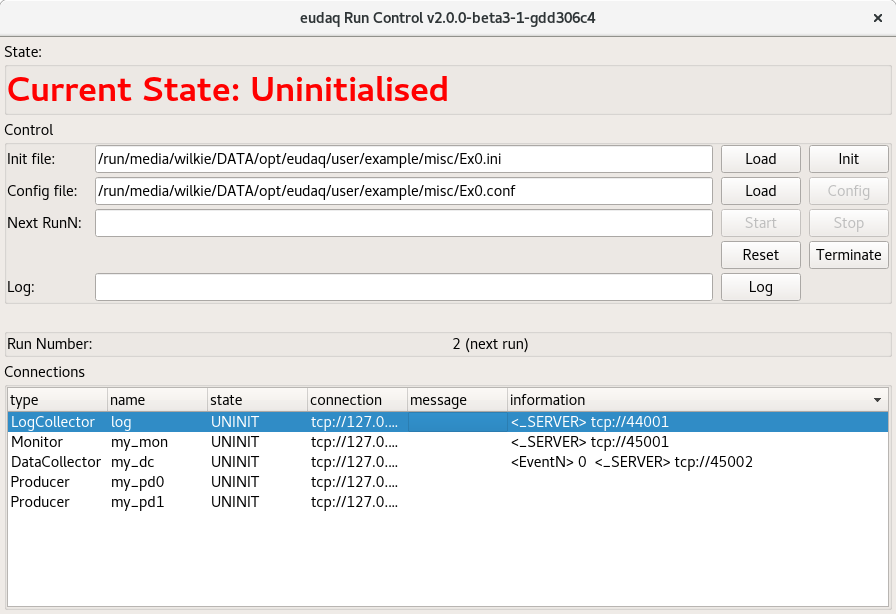
\includegraphics[width=0.8\textwidth]{src/images/eurun_ui_connected}
    \caption{The RunControl with all connections of the example setup.}
    \label{fig:RunControl_operate}
  \end{center}
\end{figure}

All of the processes report their status to the RunControl.
Depending on their status, EUDAQ and all processes can be initialized, configured or re-configured, data taking (runs) can be started and stopped, and the software can be terminated.

\begin{itemize}
\item First, the appropriate initialization file should be selected (see \autoref{sec:ConfigFiles} for creating and editing init-files). Then the \texttt{Init} button can be pressed,
which will send an initialization command to all connected processes.

\item Second, the appropriate configuration should be selected 
  (see \autoref{sec:ConfigFiles} for creating and editing configurations).
Then the \texttt{Config} button can be pressed,
which will send a configuration command
(with the contents of the selected configuration file) to all connected processes.
so that this information is always available along with the data.
\item Once all connected processes are fully configured, a run may be started, by pressing the \texttt{Start} button.
Whatever text is in the corresponding text box (``\texttt{Run:}'') when the button is pressed
will be stored as a comment in the data file.
This can be used to help identify the different runs later.
\item Once a run is completed, it may be stopped by pressing the \texttt{Stop} button.
\item At any time, a message may be sent to the log file by filling in the (``\texttt{Log:}'') text box and pressing the corresponding button.
The text should appear in the LogCollector window, and will be stored in the log file for later access.
\item Once the run is stopped, the system may be reconfigured with a different configuration, or another run may be started; or EUDAQ can be terminated.
  
\end{itemize}


\subsection{After data taking}
By default, EUDAQ provides tools to manage the the data saved in file by native EUDAQ format. Those tools could also be examples for users to write new code for more specific purpose. 
\subsubsection{Dump data}
\label{sec:dumpafterdatatacking}
To dump print Event from data file, the tool \texttt{euCliReader} is provided. The command line pattern is:
The command line pattern is:
\begin{listing}[mybash]
$[euCliReader]$ -i {input_file} -e {event_number_begin} -E {event_number_end} -tg {trigger_number_begin} -TG {tigger_number_end} -ts {timestamp_begin} -TS {timestamp_end} -s -std
\end{listing}
\begin{description}
\ttitem{-i \param{input\_file}}
required, the path of the input data file
\ttitem{-e \param{event\_number\_begin}}
optional, the low limit of event number to be printed 
\ttitem{-E \param{event\_number\_end}}
optional, the high limit of event number to be printed 
\ttitem{-tg \param{trigger\_number\_begin}}
optional, the low limit of trigger number to be printed 
\ttitem{-TG \param{trigger\_number\_end}}
optional, the high limit of trigger number to be printed 
\ttitem{-ts \param{timestamp\_begin}}
optional, the low limit of timestamp to be printed 
\ttitem{-TS \param{timestamp\_end}}
optional, the high limit of timestamp to be printed
\ttitem{-s}
optional, enable the print of statistics 
\ttitem{-std}
optional, enable the Standard Event Converter and print out StdEvent
\end{description}

The option pairs \texttt{-e -E}, \texttt{-tg -TG} and \texttt{-ts -TS} apply range limites and pick up the most intreasting Event from data file. If an option pair is not specified by user, there will be not range limit for this option pair.

\subsubsection{Convert data format}
\label{sec:convertafterdatatacking}
To convert Event from data file, the tool \texttt{euCliConverter} is provided. The command line pattern is:
The command line pattern is:
\begin{listing}[mybash]
$[euCliReader]$ -i {input_file} -o {output_file} -ip
\end{listing}
\begin{description}
\ttitem{-i \param{input\_file}}
required, the path of the input data file
\ttitem{-o \param{output\_file}}
required, the path of the output data file. 
\ttitem{-ip}
optional, enable the print of input Event 
\end{description}

If the output file has the suffix \texttt{slcio} and LCIO feature of EUDAQ is enabled at compiling time, it will generate LCIO data file.
